\def\year{2017}\relax
%File: formatting-instruction.tex
\documentclass[letterpaper]{article}
\usepackage{aaai17}
\usepackage{times}
\usepackage{helvet}
\usepackage{courier}
\frenchspacing
\setlength{\pdfpagewidth}{8.5in}
\setlength{\pdfpageheight}{11in}
\usepackage{cite}
\usepackage{subcaption}
\usepackage{hyperref}

\usepackage{graphicx}

\usepackage{titling}
\graphicspath{{figures/final/}}


\pdfinfo{
/Title (Supplementary Material: Shaping Model-Free Reinforcement Learning with Model-Based Pseudorewards)}
\setcounter{secnumdepth}{0}  
 \begin{document}
% The file aaai.sty is the style file for AAAI Press 
% proceedings, working notes, and technical reports.
%

\title{Supplementary Material: Shaping Model-Free Reinforcement Learning with Model-Based Pseudorewards}
%\subtitle{Shaping Model-Free Reinforcement Learning with Model-Based Pseudorewards}
\date{}
\maketitle

\pagebreak

\section{Experiment 3: Omniscient Dyna maze learning}

\subsection{Methods}

Whereas our method is given a full model of the environment (i.e. all state-action transition probabilities and reward contingencies), in the results presented in the main text, Dyna is not. Instead, Dyna builds a model of state-action transitions and rewards through experience. In this experiment, Dyna was given a full model of the environment. All other experimental conditions in this and all subsequent experiments were identical to those used in the experiments in the main text (e.g. the number of episodes of training, the number of simulations run, the learning rate, the discount on reward, the $\epsilon$-greedy decision policy, etc.).

\subsection{Results}

The omniscient Dyna agent learns considerably quicker than the non-omniscient agent (Figure~\ref{fig:S1a}; cf. Figure 5 in the main text), but still requires more steps (both real steps and planning steps) than the pseudoreward agent. Similarly, the CPU time required to learn the shortest path is less for the omniscient Dyna agent, although still slightly slower than the pseudoreward agent (Figure~\ref{fig:S1b}; cf. Figure 6 in the main text).

\textbf{Maze learning}

\begin{figure}[ht]
\centering
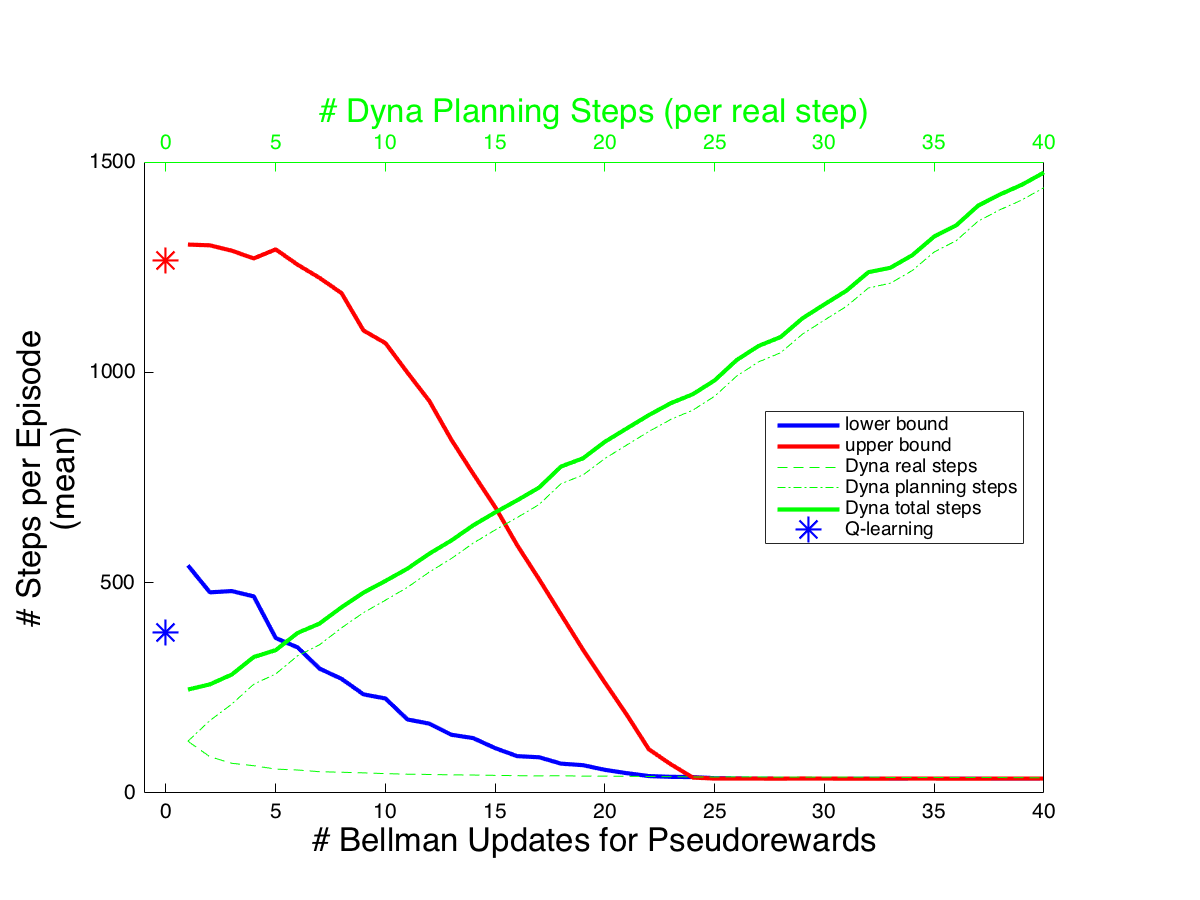
\includegraphics[width=0.5\textwidth]{learning_vs_PRiterations_omniscientDYNA_mean}
\caption{Performance of the omniscient Dyna agent in the maze environement.}
\label{fig:S1a}
\end{figure}

\begin{figure}
\centering
\begin{subfigure}{.4\textwidth}
  \centering
  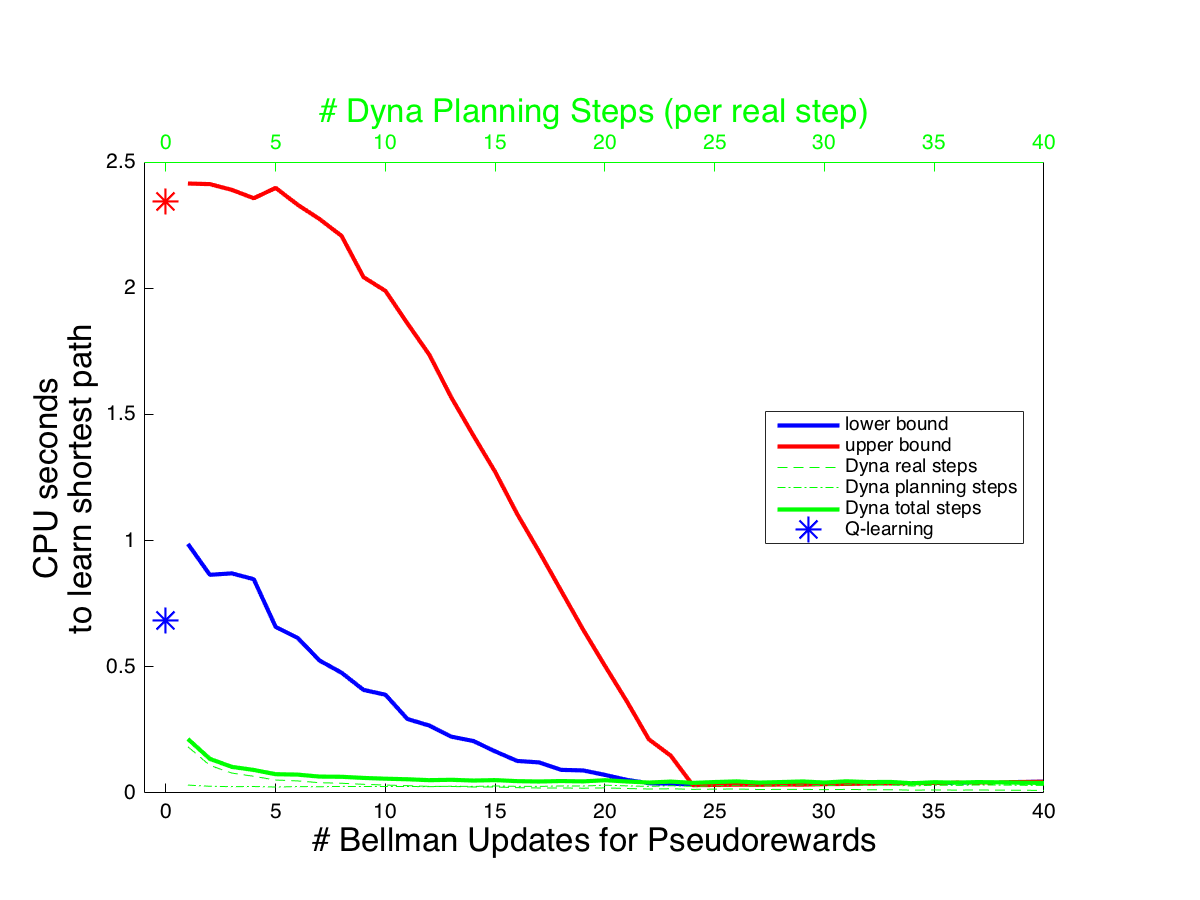
\includegraphics[width=.95\linewidth]{cpus_vs_PRiterations_omniscientDYNA_toGoal}
  \caption{}
\end{subfigure}
\begin{subfigure}{.4\textwidth}
  \centering
  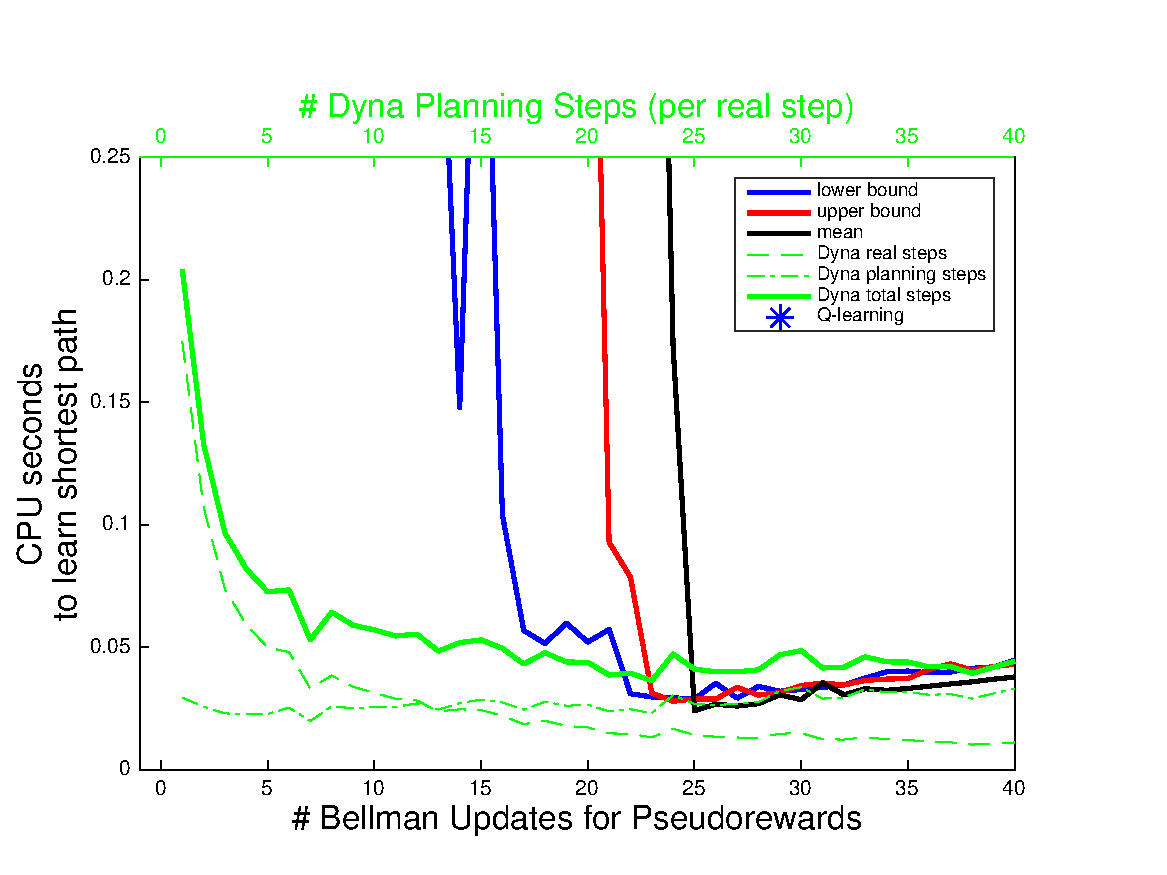
\includegraphics[width=.95\linewidth]{cpus_vs_PRiterations_omniscientDYNA_toGoal_closeup}
  \caption{Close-up of (a)}
\end{subfigure}
\caption{CPU time of the omniscient Dyna agent in the maze environement.}
\label{fig:S1b}
\end{figure}

\section{Experiment 4: Omniscient Dyna mountain car problem}

\subsection{Methods}

We also ran an experiment with an omniscient Dyna agent in a mountain car environment to compare its performance with the pseudoreward agent. All of the same parameters were used as in the experiments in the main text, the only difference being that the Dyna agent was given a full model of the environment.

\subsection{Results}

Once again, the performance improved modestly for the omniscient Dyna agent, but still required more steps to learn than the pseudoreward agent (Figure~\ref{fig:S2a}; cf. Figure 7 in the main text). Likewise, the CPU time required to learn the shortest path was less for the omniscient Dyna agent than the non-omniscient Dyna agent, but still greater than that for the pseudoreward agent (Figure~\ref{fig:S2b}; cf. Figure 8 in the main text).

\begin{figure}[ht]
\centering
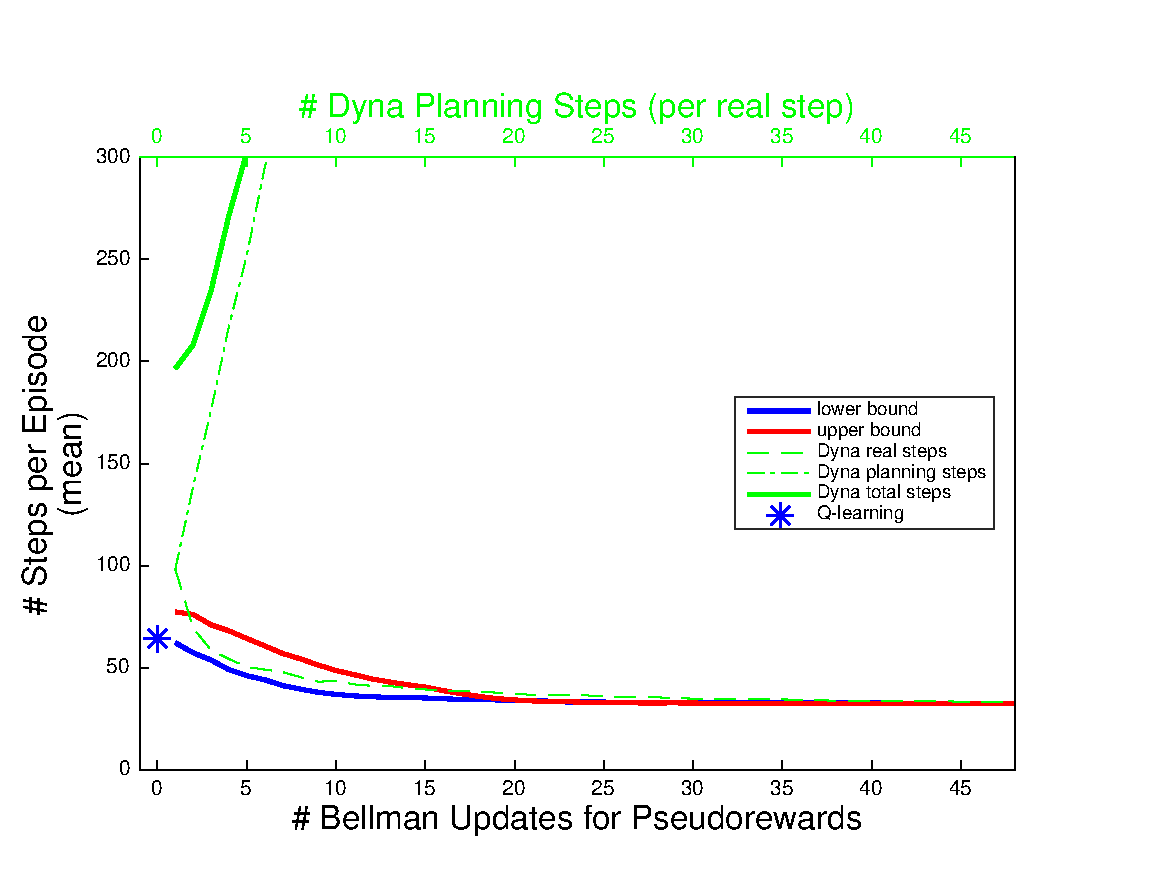
\includegraphics[width=0.5\textwidth]{MC_learning_vs_PRiterations_omniscientDYNA_mean}
\caption{Performance of the omniscient Dyna agent in the mountain car problem.}
\label{fig:S2a}
\end{figure}

\begin{figure}[ht]
\centering
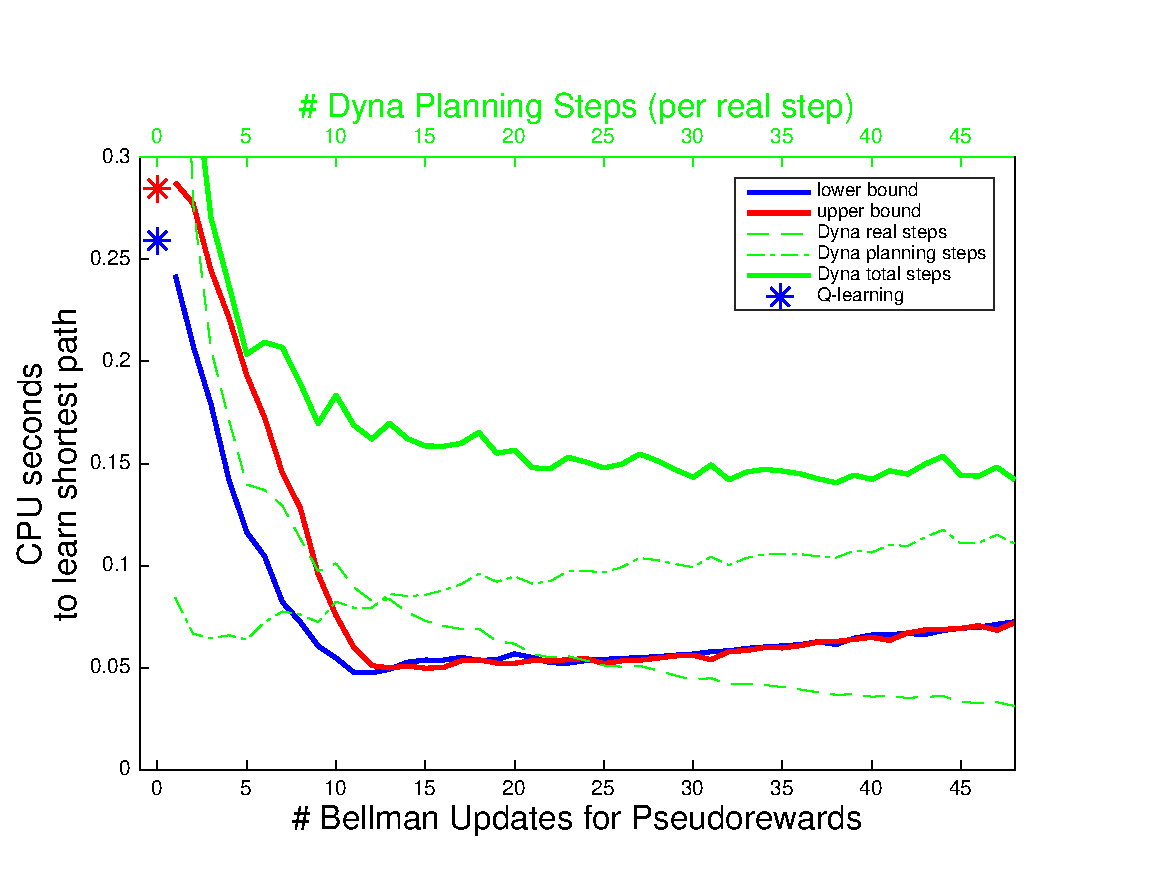
\includegraphics[width=0.5\textwidth]{MC_cpus_vs_PRiterations_omniscientDYNA_toGoal}
\caption{CPU time of the omniscient Dyna agent in the mountain car problem.}
\label{fig:S2b}
\end{figure}

\pagebreak

\section{Experiment 5: Pseudoreward method with model learning in maze environment}

\subsection{Methods}

Another way to make the pseudoreward agent more comparable to a standard Dyna agent is to have it learn a model of the environment. Just like the Dyna agent, it learns the model by storing state-action transitions and reward outcomes. Initially, it has a uniform prior overall state-action transitions and rewards, such that the probability of transitioning from any state, $s$, to any other state (or staying in the same state), $s'$, is $1/j$ where $j$ is the number of states in the environment, and the expected reward for any such transition is $R/j$, where $R$ is the expected reward for performing the task (1 for both the maze environment and the mountain car environment). Whenever the agent takes an action it replaces transition probabilities and rewards based on its experience (which is deterministic in our evironments, but this could easily be generalized to nondeterministic environments). That is, the transition probability from state $s$ to state $s'$ for action $a$ becomes one, and zero for all other states. This prior corresponds to a bimodal stick function, with sticks at zero and one. After each real step in the environment, the pseudoreward agent performs $n$ Bellman updates using its current model of the environment (or, it may perform less than $n$ iterations, based on an epsilon-optimal policy with use of span for the stopping criterion, but in practice the bound is usually $n$ after the first couple episodes of learning). These estimated state values are used to update pseudorewards after each real step.

\subsection{Results}

\textbf{Maze learning}

The number of steps required for learning is much higher in the psedoreward agent that learns a model of the environment, due to taking $n$ planning steps after each real step (Figure~\ref{fig:3a}; cf Figure 5 in the main text). However, learning still requires significantly fewer steps than than a standard (non-omniscient) Dyna agent. In terms of CPU time, on the other hand, the model-learning pseudoreward agent takes much longer to learn than the standard Dyna agent (Figure~\ref{fig:S3b}; cf. Figure 6 in the main text). This is because performing Bellman updates (requiring matrix multiplication) is about two orders of magnitude slower than performing Q-learning updates (requiring scalar multiplication only). Since $n$ iterations of the Bellman equation take place \textit{after every real step}, this computation becomes quite costly.

\begin{figure}[ht]
\centering
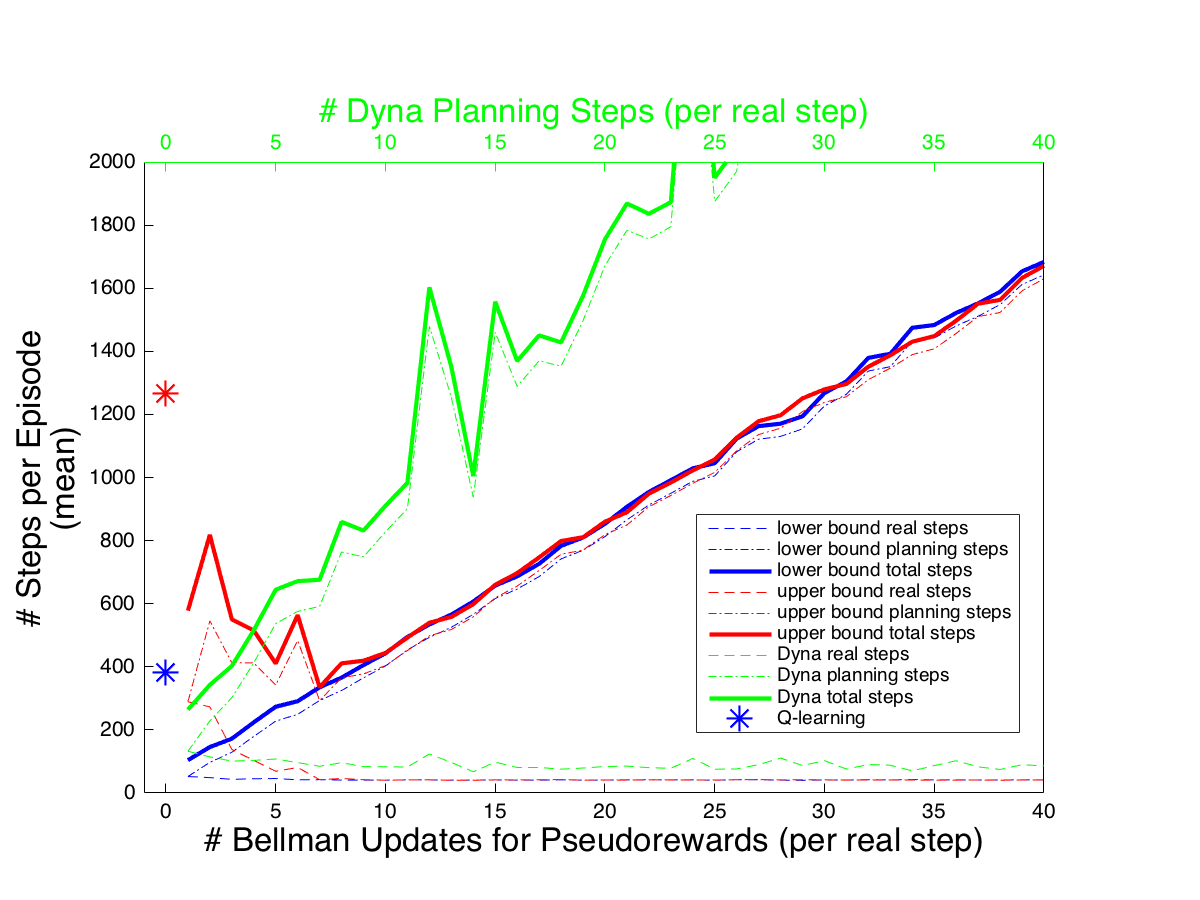
\includegraphics[width=0.5\textwidth]{learning_vs_PRiterationsLearnMod_DYNA_mean}
\caption{Performance of the model-learning pseudoreward agent in the maze environment.}
\label{fig:S3a}
\end{figure}

\begin{figure}[ht]
\centering
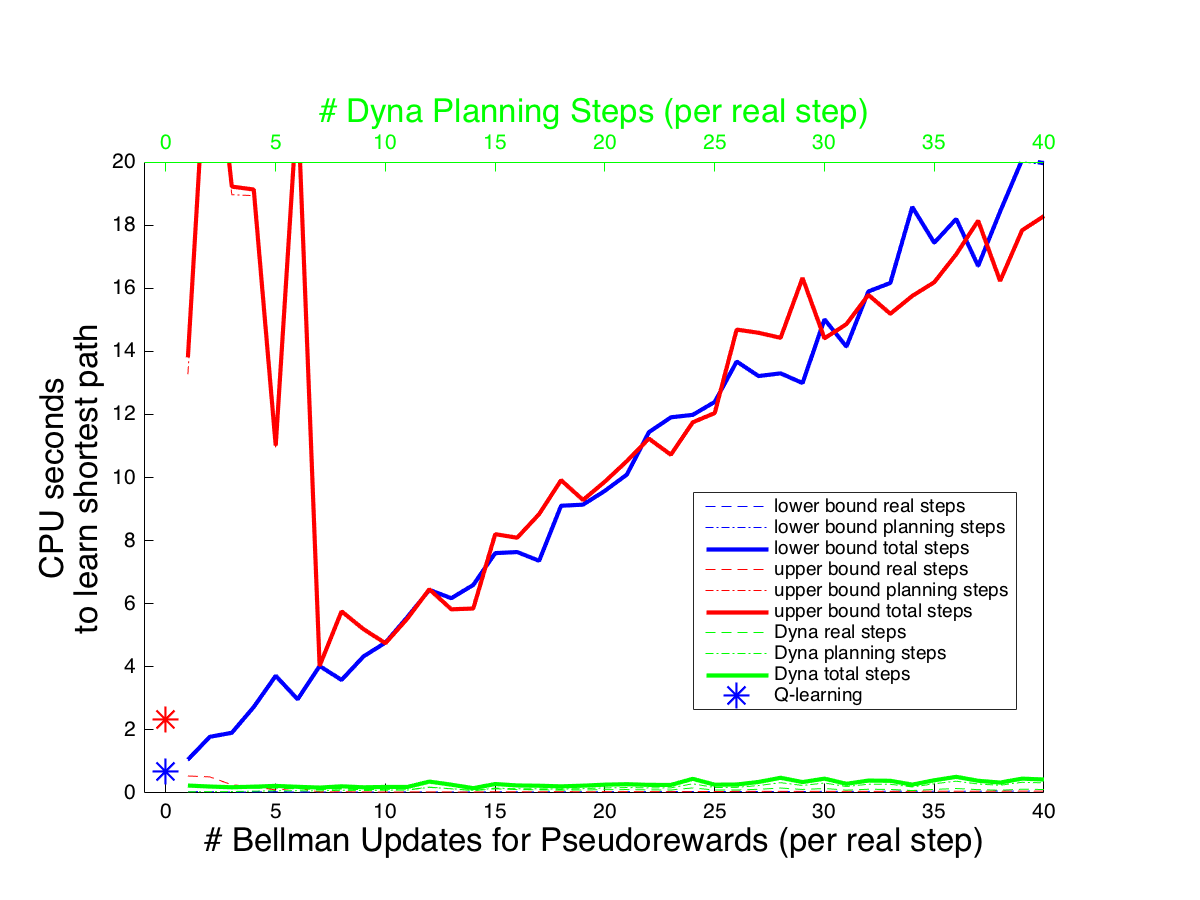
\includegraphics[width=0.5\textwidth]{cpus_vs_PRiterationsLearnMod_DYNA_toGoal}
\caption{CPU time of the model-learning pseudoreward agent in the maze environment.}
\label{fig:S3b}
\end{figure}

\section{Experiment 6: Pseudoreward method with model learning in mountain car environment}

\subsection{Methods}

The same model-learning pseudoreward agent was used in the mountain car environment and compared to a standard Dyna agent.

\subsection{Results}

As in the maze learning environment, the model-learning pseudoreward agent took many more steps to learn than the omniscient pseudoreward agent presented in the main text, but still fewer than the Dyna agent (Figure~\ref{fig:S4a}; cf. Figure 7 in the main text), and the CPU time increased drastically (Figure~\ref{fig:S4b}; cf. Figure 8 in the main text).

\begin{figure}[ht]
\centering
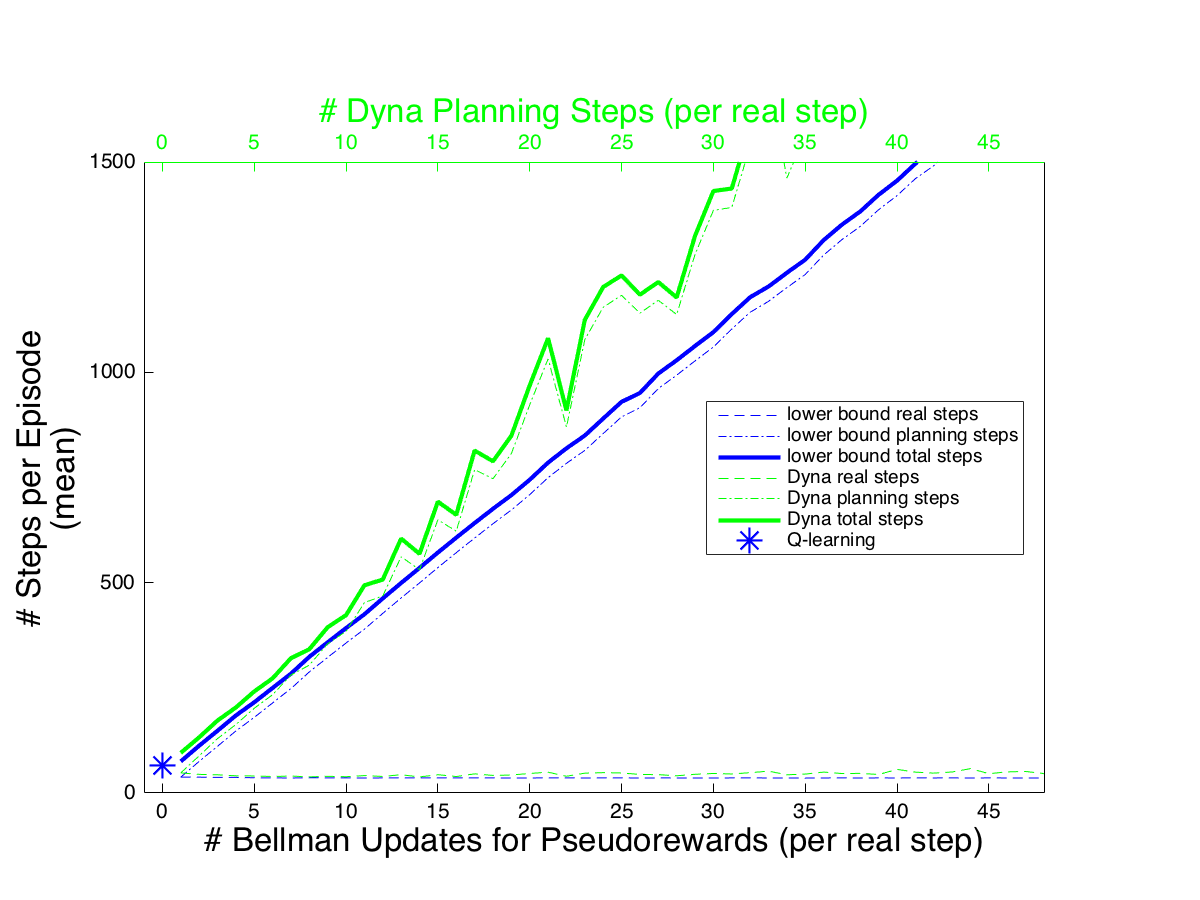
\includegraphics[width=0.5\textwidth]{MC_learning_vs_PRiterationsLearnMod_DYNA_mean}
\caption{Performance of the model-learning pseudoreward agent in the mountain car environment.}
\label{fig:S4a}
\end{figure}

\begin{figure}[ht]
\centering
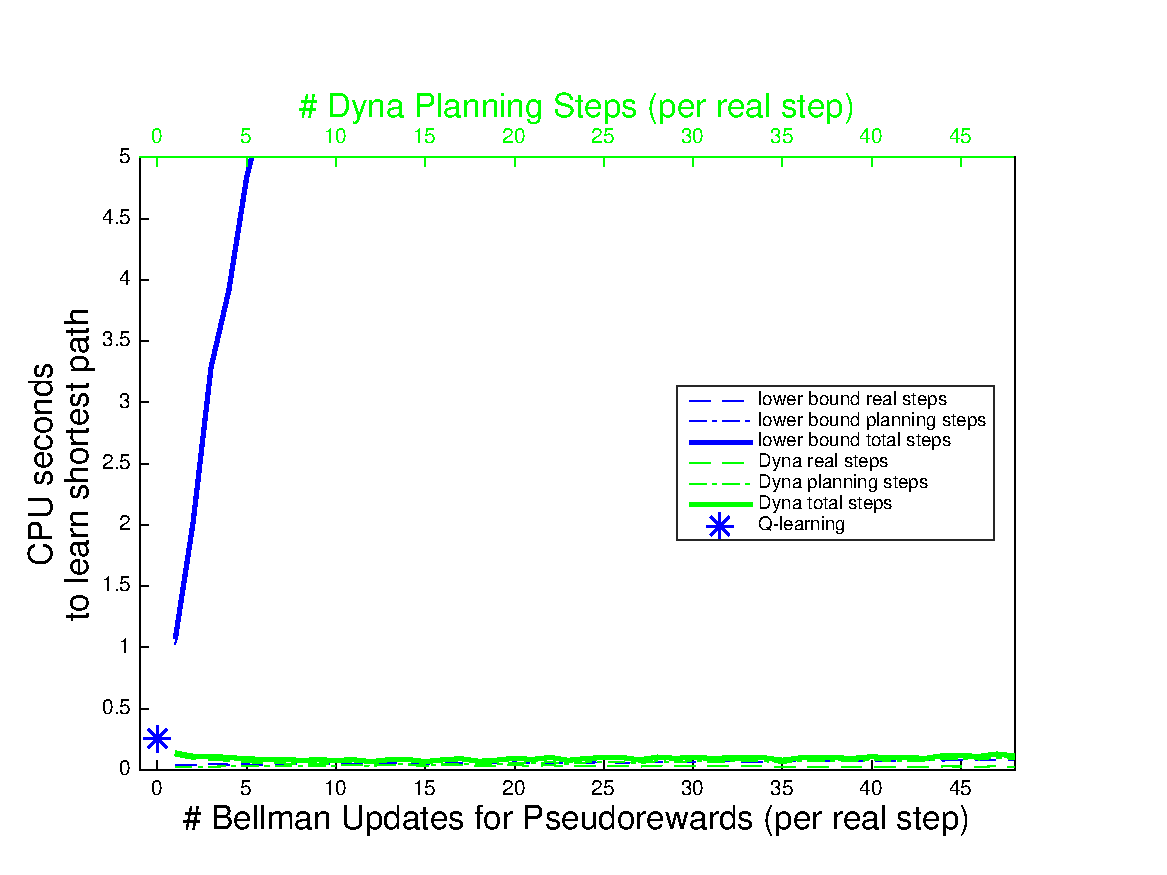
\includegraphics[width=0.5\textwidth]{MC_cpus_vs_PRiterationsLearnMod_DYNA_toGoal}
\caption{CPU time of the model-learning pseudoreward agent in the mountain car environment.}
\label{fig:S4b}
\end{figure}

\pagebreak

\section{Experiment 7: Prioritized sweeping maze learning}

\subsection{Methods}

Prioritized sweeping is a modification to the Dyna method. Like Dyna, $n$ planning steps are taken after each real step, but instead of choosing past state-action transitions at uniform random, it maintains a queue of the highest priority state-actions to replay (in practice, state-actions are only added to the queue if their temporal difference error is above some small user-defined threshold, so the number of planning steps may be less than $n$, particularly at the early stages of learning if rewards are not experienced, and in late learning when Q-values have converged). The ordering or the queue is determined by the temporal difference error from Q-learning updates. State-actions with a high temporal difference error have more uncertainty about their true state value and should therefore be replayed before states with less uncertainty. Prioritized sweeping usually includes model-learning, just like the standard Dyna agent. However, it could also be omniscient with respect to all state-action transition probabilities and reward contingencies. An omniscient prioritized sweeping agent would require $d$ steps of Q-learning to learn Q-values that guide the agent to the goal from state $s$, where $d$ is the distance from state $s$ to the goal. However, as soon as a non-omniscient prioritized sweeping agent reaches the goal, it too can acheive this with $d$ steps of Q-learning; while it wouldn't have a full model of the environment it would have enough information to guide along the shortest path to the goal from any state that it has already visited.

\subsection{Results}

While prioritized sweeping learns more quickly than a Dyna agent, it still requires many more steps than the pseudoreward agent, due to planning (Figure~\ref{fig:S5a}; cf. Figure 5 in the main text). Its CPU time is also very high (Figure~\ref{fig:S5b}; cf. Figure 6 in the main text). Prioritized sweeping especially suffers from the computation time required to sort the queue after every planning step.

\begin{figure}[ht]
\centering
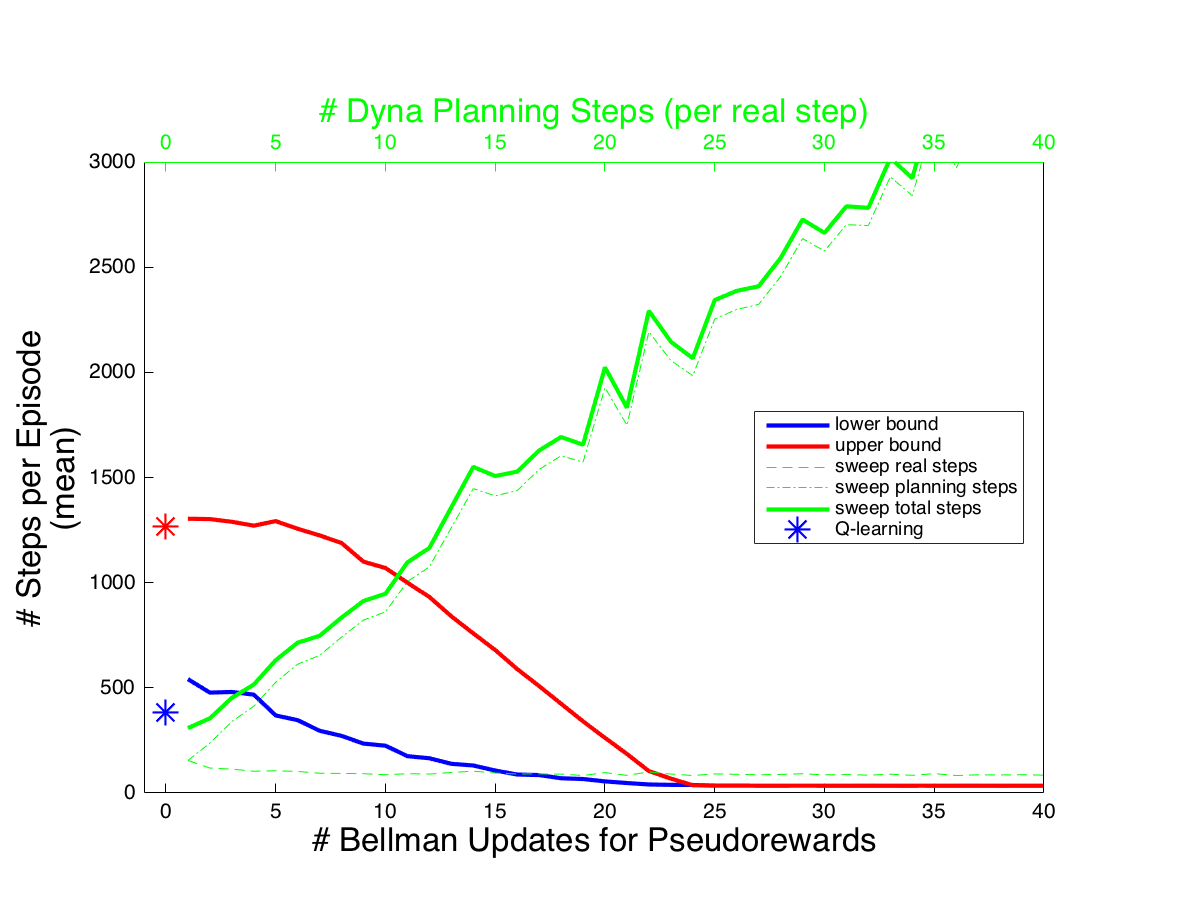
\includegraphics[width=0.5\textwidth]{learning_vs_PRiterationsSweeping_DYNA_mean}
\caption{Performance of the prioritized sweeping agent in the maze environment.}
\label{fig:S5a}
\end{figure}

\begin{figure}[ht]
\centering
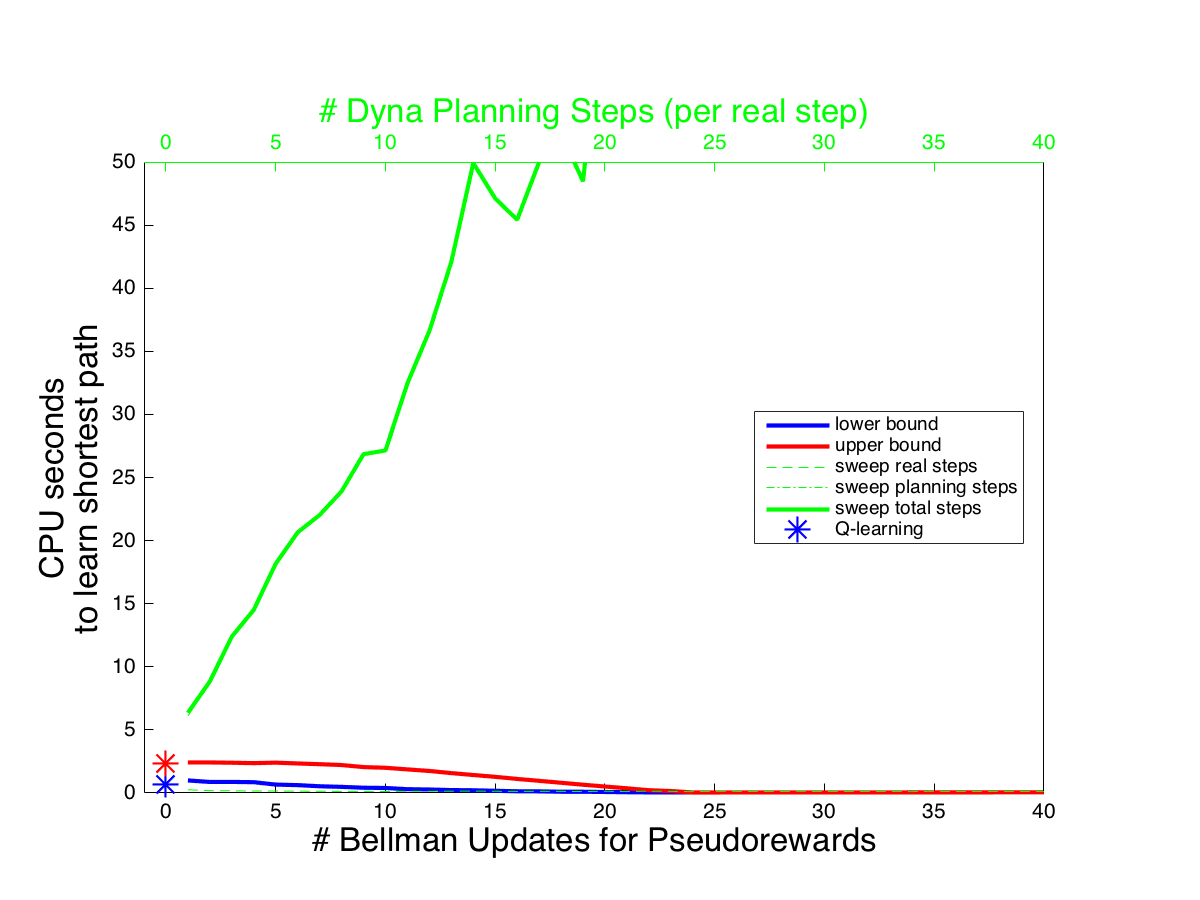
\includegraphics[width=0.5\textwidth]{cpus_vs_PRiterations_sweeping_toGoal}
\caption{CPU time of the prioritized sweeping agent in the maze environment.}
\label{fig:S5b}
\end{figure}

\section{Experiment 8: Prioritized sweeping mountain car problem}

\subsection{Methods}

The same prioritized sweeping algorithm was used in the mountain car environment and compared to the pseudoreward agent.

\subsection{Results}

Once again, the prioritized sweeping agent is an improvement from a Dyna agent, but requires many more steps (Figure~\ref{fig:S6a}; cf. Figure 7 in the main text) and CPU time (Figure~\ref{fig:S6b}; cf. Figure 8 in the main text) than the pseudoreward agent.

\begin{figure}[ht]
\centering
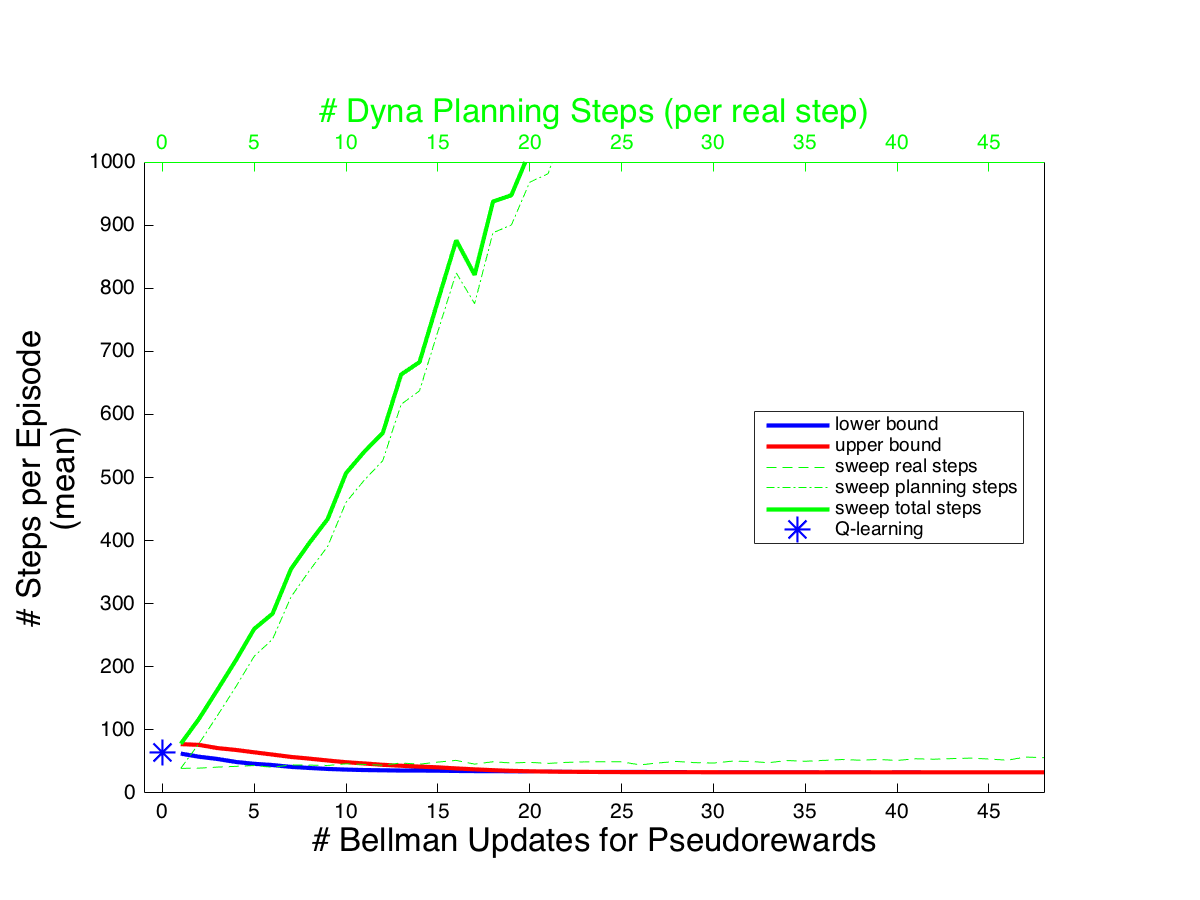
\includegraphics[width=0.5\textwidth]{MC_learning_vs_PRiterationsSweeping_DYNA_mean}
\caption{Performance of the prioritized sweeping agent in the mountain car environment.}
\label{fig:S6a}
\end{figure}

\begin{figure}[ht]
\centering
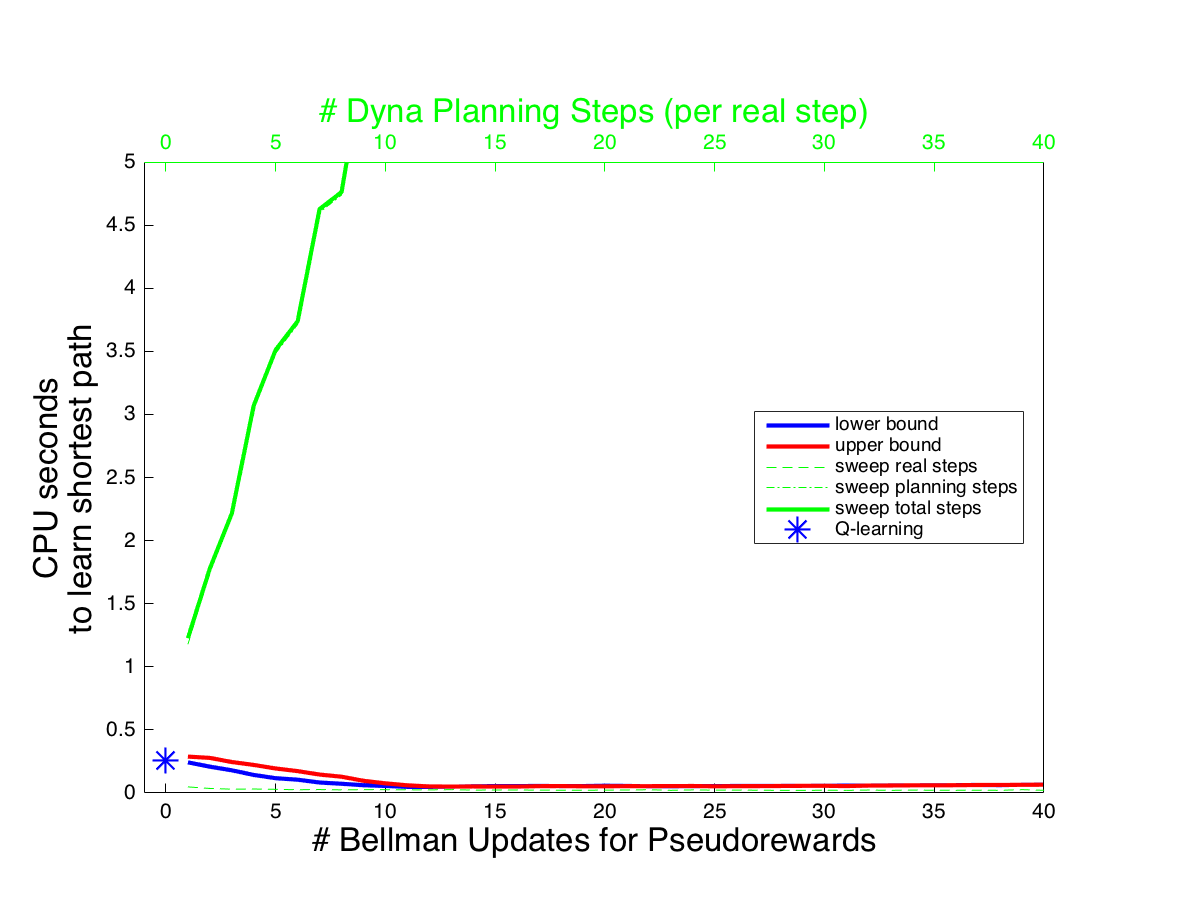
\includegraphics[width=0.5\textwidth]{MC_cpus_vs_PRiterations_sweeping_toGoal}
\caption{CPU time of the prioritized sweeping agent in the mountain car environment.}
\label{fig:S6b}
\end{figure}

\end{document}
